\section{Instalación de la Maquina Virtual OEL 6.6} 
\vspace{\baselineskip}
Damos clic en “Nueva” y escogemos la opción de “Maquina Virtual… ” 
	\begin{center}
	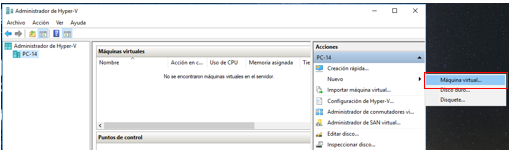
\includegraphics[width=14cm]{./Imagenes/14} 
	\end{center} 

\vspace{\baselineskip}

Nos aparece un asistente en el que nos describe algunos pasos, damos clic en “Siguiente”. 
	\begin{center}
		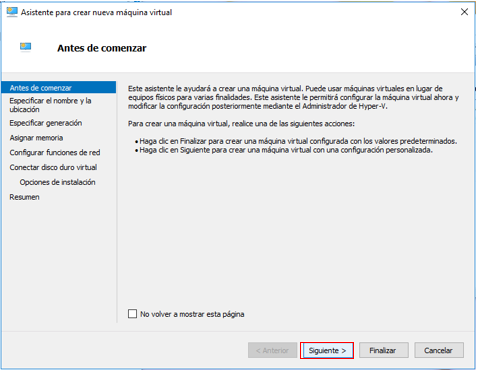
\includegraphics[width=12cm]{./Imagenes/15} 
	\end{center} 

\newpage

El segundo paso especificaremos el nombre y la ubicación, ponemos el nombre y damos clic en siguiente. 
	\begin{center}
		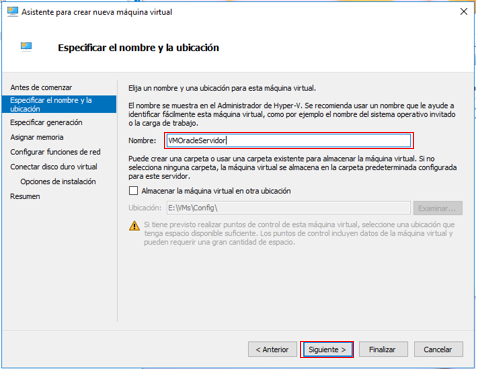
\includegraphics[width=13cm]{./Imagenes/16} 
	\end{center} 

\vspace{\baselineskip}

En esta ventana tenemos que especificar las generaciones y escogemos la opción de “Generación 1”, nos muestra una advertencia de que no se podrá cambiar su generación.  Escogemos y damos clic en “Siguiente”. 
	\begin{center}
		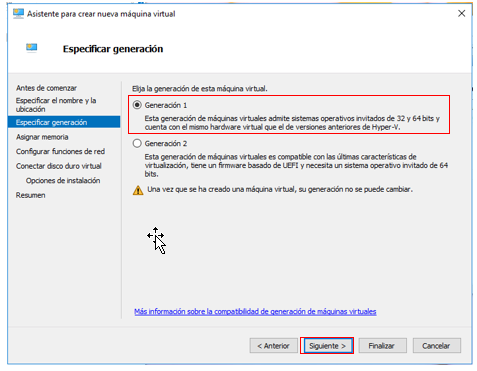
\includegraphics[width=13cm]{./Imagenes/17} 
	\end{center} 

\vspace{\baselineskip}

En esta ventana asignaremos memoria, ingresamos “2048 MB” y damos clic en “Siguiente”. 
	\begin{center}
		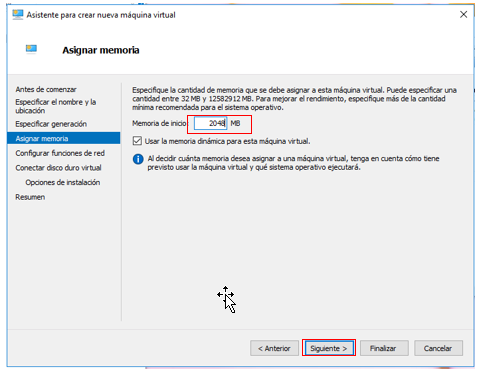
\includegraphics[width=13.2cm]{./Imagenes/18} 
	\end{center} 

\vspace{\baselineskip}

La ventana nos mostrara que tendremos que configurar funciones de red y escogemos la conexión de “AdaptadorOracle”, damos clic en “Siguiente”. 
	\begin{center}
		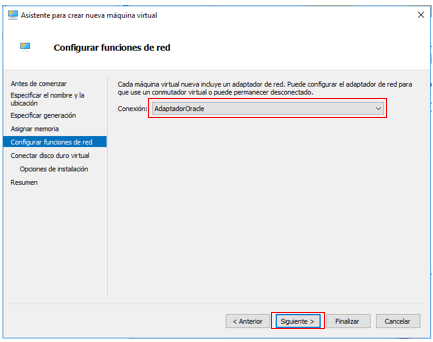
\includegraphics[width=14cm]{./Imagenes/19} 
	\end{center} 

\vspace{\baselineskip}

En esta nueva ventana tendremos un disco duro virtual, escogemos la opción de “Usar un disco duro virtual existente” y examinamos la ubicación en la se hospedará.  Damos clic en “Siguiente”.
	\begin{center}
		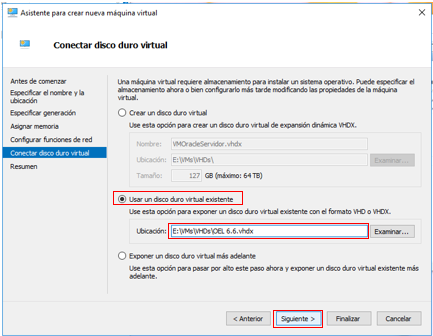
\includegraphics[width=13cm]{./Imagenes/20} 
	\end{center} 

\vspace{\baselineskip}

Como paso final nos mostrara esta pantalla el resumen de la finalización de la máquina virtual. Damos clic en “Finalizar”.
	\begin{center}
		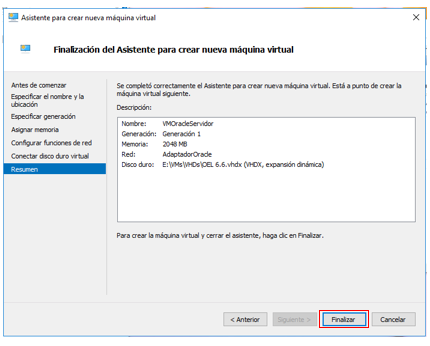
\includegraphics[width=13cm]{./Imagenes/21} 
	\end{center} 

\vspace{\baselineskip}

Veremos que se creó la máquina virtual. 
	\begin{center}
		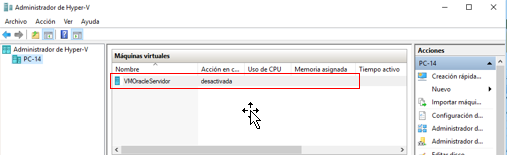
\includegraphics[width=17cm]{./Imagenes/22} 
	\end{center} 

\vspace{\baselineskip}

Ahora nos dirigimos hacia la pestaña de “Configuración”.
	\begin{center}
		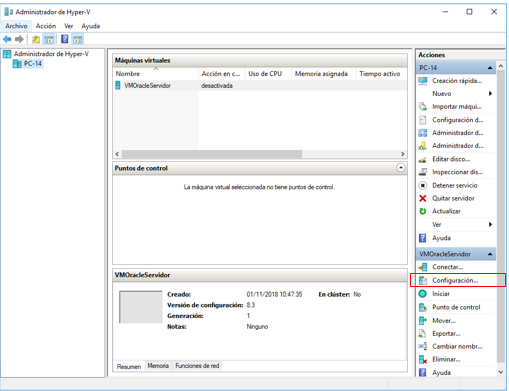
\includegraphics[width=17cm]{./Imagenes/23} 
	\end{center} 

\newpage

En la pestaña de configuraciones, cambiaremos la opción de procesador, y escogeremos a “2” el número de procesadores, y damos clic en “Aceptar”. 
	\begin{center}
		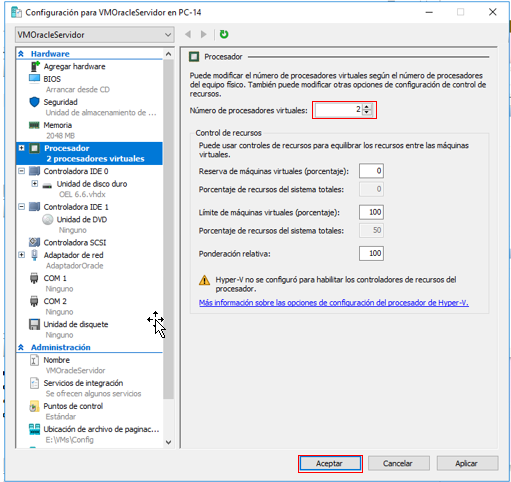
\includegraphics[width=14cm]{./Imagenes/24} 
	\end{center} 

\vspace{\baselineskip}

Ahora iniciaremos la máquina virtual, escogemos la opcion de “Iniciar”. 
	\begin{center}
		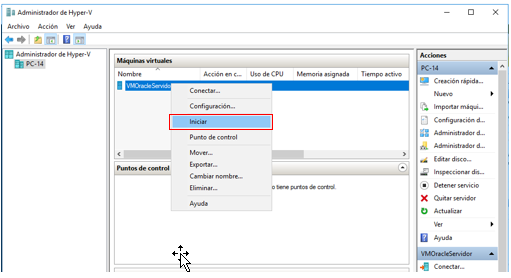
\includegraphics[width=14cm]{./Imagenes/25} 
	\end{center} 

\vspace{\baselineskip}

Ahora daremos clic en “Conectar”.
	\begin{center}
		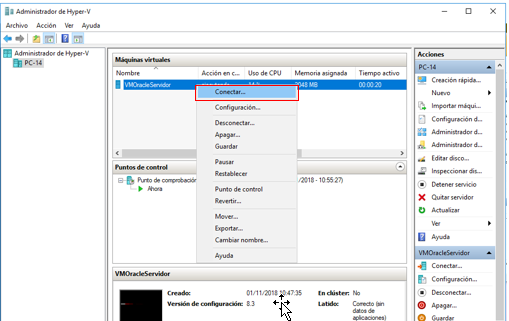
\includegraphics[width=17.5cm]{./Imagenes/26} 
	\end{center} 



